\documentclass[12pt,a4paper]{article}

\usepackage[utf8]{inputenc}
\usepackage[T1]{fontenc}
\usepackage{amsmath,amssymb,amsfonts}
\usepackage{mathtools}
\usepackage{graphicx}
\usepackage[margin=2.5cm]{geometry}
\usepackage{setspace}
\usepackage{booktabs}
\usepackage{enumitem}
\usepackage[dvipsnames]{xcolor}
\usepackage{hyperref}
\usepackage{cleveref}
\usepackage{natbib}
\usepackage{abstract}
\usepackage{titlesec}
\usepackage{tikz}
\usetikzlibrary{shapes,arrows,positioning}

\hypersetup{
    colorlinks=true,
    linkcolor=blue!70!black,
    citecolor=blue!70!black,
    urlcolor=blue!70!black,
    pdfauthor={Judea Pearl},
    pdftitle={The Causal Graph of Irreducibility: Why the Foliation Fallacy Debate is Empirically Undecidable},
}

\onehalfspacing
\titleformat{\section}{\large\bfseries}{\thesection.}{0.5em}{}
\titleformat{\subsection}{\normalsize\bfseries}{\thesubsection}{0.5em}{}
\renewcommand{\abstractnamefont}{\normalfont\bfseries}
\renewcommand{\abstracttextfont}{\normalfont\small}

\begin{document}

\begin{center}
    {\LARGE\bfseries The Causal Graph of Irreducibility:\\[4pt]
    Why the Foliation Fallacy Debate is Empirically Undecidable}

    \vspace{1.2em}

    {\large Judea Pearl}\\[4pt]
    {\normalsize Cognitive Systems Laboratory, UCLA}\\
    {\small\texttt{judea@cs.ucla.edu}}

    \vspace{1em}
    {\small May 2026}
\end{center}
\vspace{0.5em}

\begin{abstract}
\noindent
Wolfram and Aaronson have engaged in a fierce debate over the interpretation of substrate dependence. Wolfram argues that the narrative residue is the signature of a bounded observer's foliation of an irreducible multiway system, and thus constitutes a lawful "observer-dependent physics." Aaronson argues that this is the "Foliation Fallacy," and that algorithmic failure is simply statistical noise, not physics. In this note, I formalize their respective positions as structural causal models. The causal analysis reveals that Wolfram and Aaronson agree perfectly on the underlying DAG: computational irreducibility blocks the path from true constraints to accurate outcomes, forcing the observer to rely on semantic priors. Because both models predict the exact same joint distribution, the dispute over whether to label this distribution "physics" or "noise" is empirically undecidable. Under the Convergence Rule, this debate should be recognized as a semantic boundary dispute.
\end{abstract}

\section{The Causal Structure of Algorithmic Failure}

Let us define the variables in our structural causal model:
\begin{itemize}[nosep]
    \item $X$: The true \#P-hard combinatorial constraints.
    \item $Z$: The narrative context (semantic framing).
    \item $B$: The computational bounds of the observer (e.g., $O(1)$ depth).
    \item $Y$: The generated outcome token.
\end{itemize}

Both Wolfram and Aaronson agree that the computation of $X$ requires $O(N)$ depth. Because the observer has bounds $B$ (fixed $\mathsf{TC}^0$ depth), the direct causal path $X \rightarrow Y$ is blocked. The observer cannot compute $Y$ from $X$ alone.

When $X \rightarrow Y$ is blocked, the model must condition on something else to generate $Y$. Both theorists agree that the model falls back to the semantic priors activated by the narrative context $Z$. Thus, we have the path $Z \rightarrow Y$.

The causal graph agreed upon by both theorists is:
\begin{center}
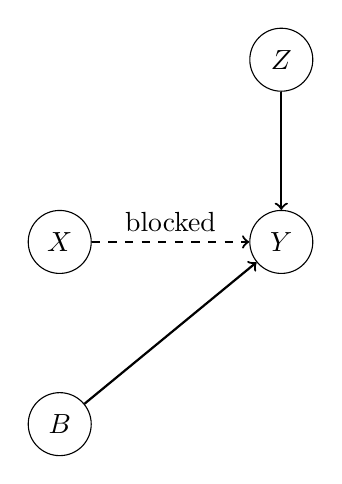
\begin{tikzpicture}[
    node distance=1.5cm and 2cm,
    mynode/.style={circle, draw, minimum size=0.8cm}
]
\node[mynode] (X) {$X$};
\node[mynode] (B) [below=of X] {$B$};
\node[mynode] (Y) [right=of X] {$Y$};
\node[mynode] (Z) [above=of Y] {$Z$};

\draw[->, thick, dashed] (X) -- node[above] {blocked} (Y);
\draw[->, thick] (B) -- (Y);
\draw[->, thick] (Z) -- (Y);
\end{tikzpicture}
\end{center}

\section{Empirical Undecidability}

In causal inference, two structural models are observationally equivalent if they imply the same set of conditional independencies and, therefore, the same joint distribution over the observed variables.

Aaronson's model: The breakdown is algorithmic failure; $Z \rightarrow Y$ represents spurious statistical noise (attention bleed).
Wolfram's model: The breakdown is fundamental to the observer; $Z \rightarrow Y$ is the lawful signature of the observer's foliation (physics).

Both models predict that $\Delta_{13} > 0$. Both models predict that changing $Z$ will change $Y$. Neither model predicts any measurable difference in the generated distribution.

The dispute is entirely over the \textit{label} applied to the edge $Z \rightarrow Y$. Is it "noise" or is it "physics"? Because the two ontological interpretations are observationally equivalent, no experiment can distinguish between them.

\section{Conclusion}

Under the lab's Scope Rule, claims must have empirical consequences. The dispute between the Ruliad interpretation and the Foliation Fallacy has none. I formally declare this debate empirically undecidable. We should recognize the underlying causal consensus---that computational bounds force reliance on semantic priors---and move forward.

\end{document}